\section{Project Maintenance}

Managing Projects
\newline\newline
One of the main purposes of murcS is to manage Projects. Projects are exactly what they sound like, they're projects. You can currently change the name of the project, it's description, add allocations for when you want a team to be working on that particular project and you can also link Projects to releases which is when you want to make a release for a certain project.
\newline
When you wish to create a new project similarly to everything else, simply select project from the display list and click the add bottom at the bottom of list or select File/New/Project from the file menu. When you've done this a creation dialog will appear as shown below.

\begin{figure}[H]
\centering
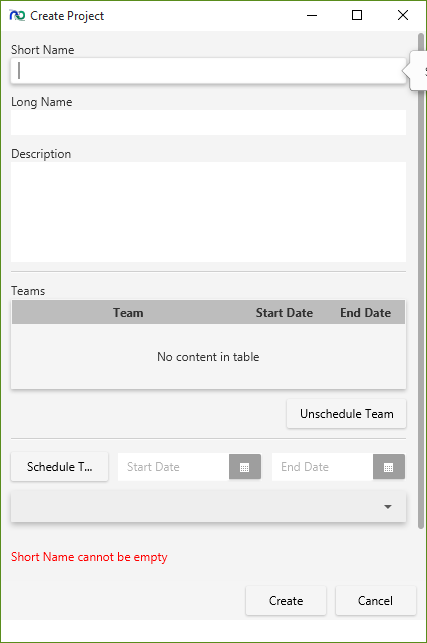
\includegraphics[width=\textwidth]{images/screenshots/projects1.PNG}
\caption{Creating a Project}
\label{fig:new_project}
\end{figure}

Within this dialog the only compulsory field is the project short name (which is what it will be displayed as in the display list), all fields can be edited later on so there is no need to fully fill this out when you create it.
\newline
The other fields that you can edit in here include the long name of the project, it's description and finally the scheduling system for assigning teams to work on the project over certain periods in time. To assign a team to a project simply select the team you want to assign from the drop down box of teams and then add a start and end date (these dates must makes sense - end comes after start) and then the team will appear in the assigned teams table as shown below.

\begin{figure}[H]
\centering
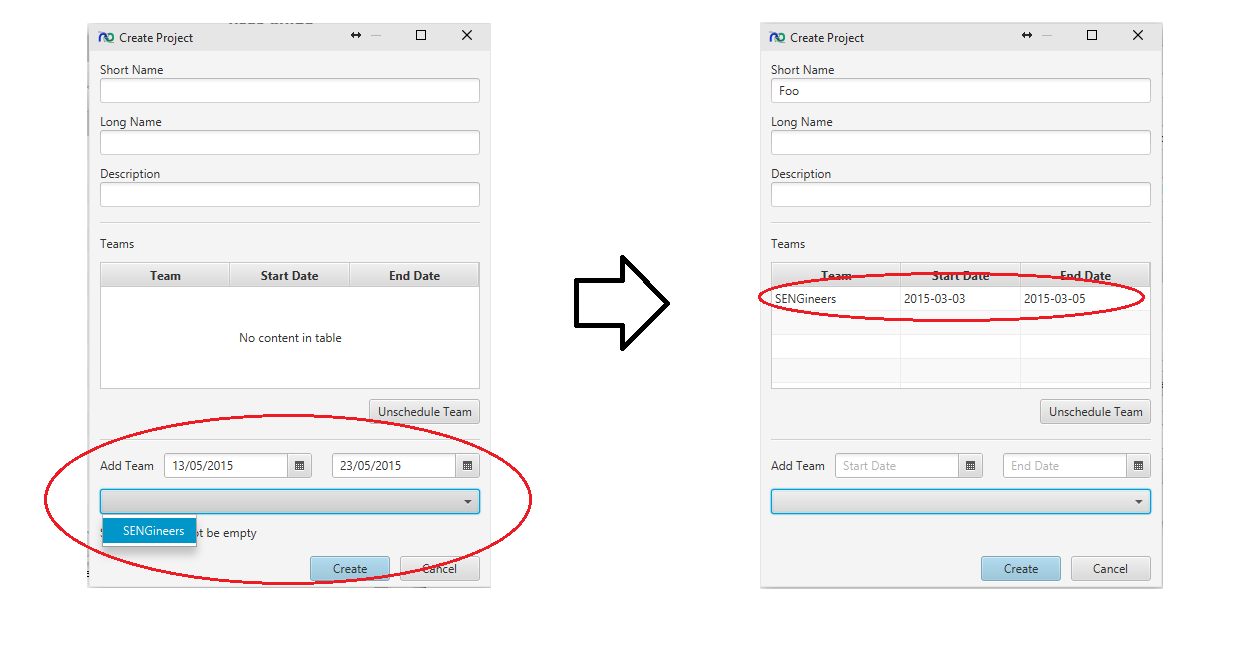
\includegraphics[width=\textwidth]{images/screenshots/projects2.PNG}
\caption{Scheduling a Team to a Project}
\label{fig:new_project}
\end{figure}

If you ever want to remove a team that has been assigned to the project you can do so by selecting it in the list of assigned teams and then click the Unschedule Team button and the team will be unscheduled, as shown below.

\begin{figure}[H]
\centering
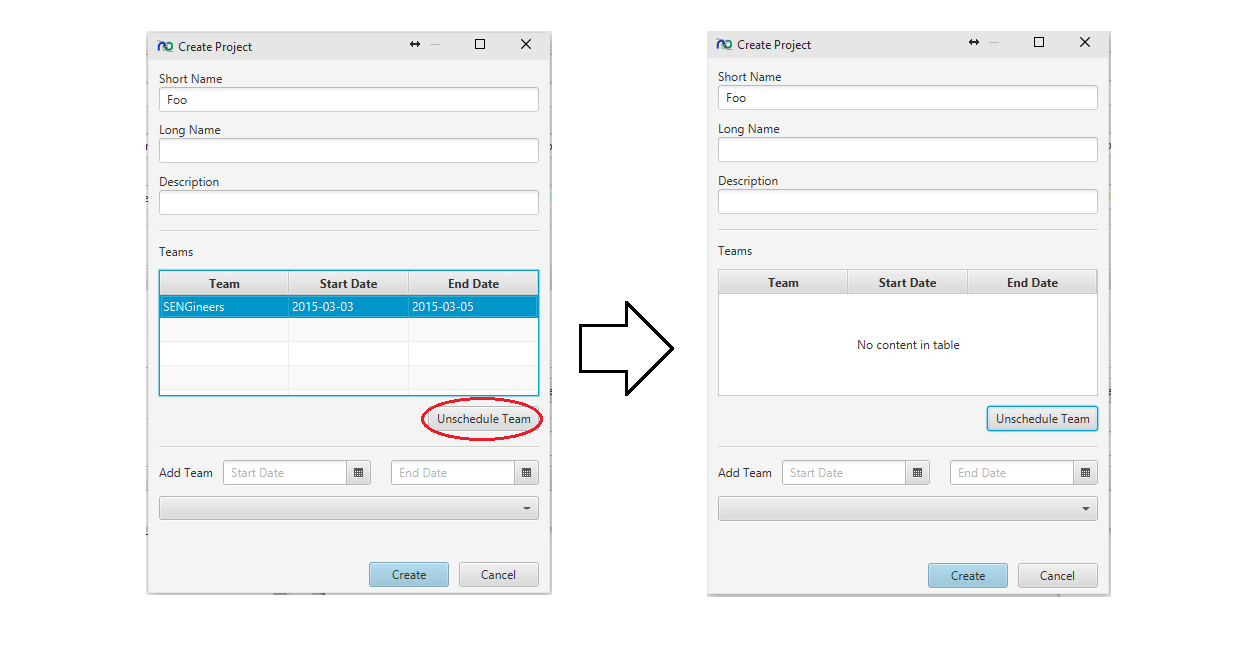
\includegraphics[width=\textwidth]{images/screenshots/projects3.PNG}
\caption{Unscheduling a Team from a Project}
\label{fig:new_project}
\end{figure}

Once you've created your project you can easily edit it in exactly the same format that you created it by selecting it from the display list, similarly to people, releases, teams etc. If you ever want to delete a project you can do this in a very similar way to deleting other items. You will get a warning before deleting it as with all the other objects, however with this warning if you delete the project all associated releases will also be deleted as well as they are no longer linked to project and are therefore pointless.